\documentclass[12pt]{exam}
\usepackage[utf8]{inputenc}
\usepackage[a4paper,top=2cm,left=2cm,right=2cm,bottom=2cm]{geometry}
\usepackage{import}
\usepackage[T1]{fontenc}
\usepackage[german,ngerman]{babel}
\usepackage[table]{xcolor}
\usepackage{amsthm, esvect}
\usepackage{mathtools}
\RequirePackage{amssymb, amsfonts, amsmath, latexsym, verbatim, xspace}
\usepackage{systeme}
\usepackage{multicol}
\usepackage{multirow}
\usepackage{framed}
\usepackage{array}
\usepackage{ragged2e}
\usepackage{graphicx}
\usepackage{pdflscape}
\usepackage{epstopdf}
\usepackage{booktabs}
\usepackage{pdfpages}
\usepackage{float} % Allows putting an [H] in \begin{figure} to specify the exact location of the figure
\usepackage{wrapfig} % Allows in-line images such as the example fish picture
\usepackage{tikz, graphicx} % tikz
\usepackage[position=top]{subfig}
\usepackage[bookmarks=true]{hyperref}%Links
\usepackage{enumerate}
\usepackage{enumitem}
\usepackage[german,ruled,vlined,linesnumbered,algosection]{algorithm2e}
\usepackage[labelfont=sf]{caption}
\usepackage{lmodern}
\usepackage{lscape}
\usepackage{tabularx}
\usepackage{systeme}
\usepackage{hhline}
\usepackage{subfiles}
\usepackage{stackengine}
\usepackage{setspace}
\usepackage{MnSymbol}
\usepackage{tcolorbox}
\usepackage{bbm}
\usepackage{url}
\usepackage{xparse}
\usepackage{sectsty}
\usepackage{array}
\usepackage{ragged2e}
\usepackage{listings} %Stellt Code-Snippets sauber dar

% definiert die Sprache
\selectlanguage{German}

% add command for different dates in Swiss fashion
\newcommand{\monthwordlong}[1]{\ifcase#1 \or Januar\or Februar\or März\or April\or Mai\or Juni\or Juli\or August\or September\or Oktober\or November\or Dezember\fi}
\newcommand{\monthwordshort}[1]{\ifcase#1\or Jan\or Feb\or Mar\or Apr\or Mai\or Jun\or Jul\or Aug\or Sept\or Okt\or Nov\or Dez\fi}
\newcommand{\datelong}{\number\day.\:\monthwordlong{\the\month}\:\number\year}
\newcommand{\dateshort}{\number\day.\:\monthwordshort{\the\month}\:\number\year}

% define color of links inside a text
\definecolor{linkblue}{RGB}{0, 0, 80}
\definecolor{plotblue}{RGB}{100, 100, 255}
\definecolor{myblue}{RGB}{8,164,214}
\definecolor{myred}{RGB}{143,42,41}
\definecolor{forestgreen}{RGB}{34,139,34}
\definecolor{highdive}{RGB}{10,169,194}
\definecolor{charcoal}{RGB}{74,74,74}
\hypersetup{
	colorlinks=true,
	linkcolor=linkblue,
	filecolor=magenta,
	urlcolor=plotblue,
	citecolor=linkblue,
	pdfpagemode=FullScreen,
}


\lstdefinestyle{mystyle}{ % definiert den style des Code-Snippets
	%backgroundcolor=\color{backcolour},
	%commentstyle=\color{codegreen},
	%keywordstyle=\color{magenta},
	%numberstyle=\tiny\color{codegray},
	%stringstyle=\color{codepurple},
	basicstyle=\ttfamily\footnotesize,
	breakatwhitespace=false,
	breaklines=true,
	captionpos=b,
	keepspaces=true,
	%numbers=left,
	%numbersep=5pt,
	showspaces=false,
	showstringspaces=false,
	showtabs=false,
	tabsize=4
}
\lstset{style=mystyle}
\qformat{\Large\textbf{Aufgabe \thequestion\hfill\thepoints}}
\newlist{partes}{enumerate}{3}
\setlist[partes]{label=(\alph*)}
\newcommand{\parte}{\item}
\newlist{subpartes}{enumerate}{3}
\setlist[subpartes]{label=\roman*)}
\newcommand{\subparte}{\item}
\setlist[enumerate,1]{%(
	leftmargin=*, itemsep=12pt, label={\textbf{\arabic*.)}}}
\newcommand\answerbox{%%
	\fbox{\rule{2in}{0pt}\rule[-0.1ex]{0pt}{4ex}}}
\pointpoints{Punkt}{Punkte}
\hqword{Frage:}
\hpword{Mögliche Punkte:}
\hsword{Erreicht:}
\htword{Total}
\renewcommand*\half{.5}
\renewcommand{\solutiontitle}{\noindent\textbf{Lösung:}\par\noindent}

% Graphed boxes
\newcommand{\karos}[2]{
  \begin{tikzpicture}
    \draw[step=0.4cm,color=cyan,dotted] (0,0) grid (#1 cm ,#2 cm);
  %  \draw((#1)/2 cm,0)--((#1)/2 cm,/#2)/2cm)
  \end{tikzpicture}
}
\usetikzlibrary{arrows, petri, topaths, graphs}
\linespread{1.2} % Line spacing

%=========================================================
\newenvironment{parcols}[1][]{
    \begin{parts}\begin{multicols}{#1}
}{
    \end{multicols}\end{parts}
}
%=========================================================
\newenvironment{itemcols}[1][]{
	\begin{itemize}\begin{multicols}{#1}
		}{
	\end{multicols}\end{itemize}
}

%=========================================================
\newcommand{\antwort}[1]{
	{\setlength{\textwidth}{\textwidth}\fillwithgrid{#1cm}\vspace{5pt}}
}

%=========================================================
% Karriertes Papier für Antwort MIT OVERLAY
\tcbuselibrary{breakable,skins}
\usetikzlibrary{mindmap,trees}
\newlength\tindent
\setlength{\tindent}{\parindent}
\setlength{\parindent}{0pt}
\setlength{\parskip}{0pt}

\newtcolorbox{gridspace}[1]{%
	enhanced,
	breakable,
	blanker,
	boxrule=0pt,
	left=5mm,
	right=5mm,
	top=5.75mm,
	bottom=0mm,
	boxsep=0pt,
	height=#1cm,
	width=16cm,
	before upper={
		\begingroup
		\setlength{\baselineskip}{5.75mm}
		\setlength{\parskip}{0pt}
		\setlength{\lineskip}{0pt}
		% keep every paragraph on the grid rhythm
		%\everypar{\vspace{0pt}\strut}
		% math formulas shifted by one grid row
		\let\oldbracketopen\[
		\renewcommand{\[}{\vspace{-5mm}\oldbracketopen}
		% Align displayed formulas to the grid
		\setlength{\abovedisplayskip}{0pt}
		\setlength{\belowdisplayskip}{0pt}
		\setlength{\abovedisplayshortskip}{0pt}
		\setlength{\belowdisplayshortskip}{0pt}
		% Enumerate follows the same rhythm
		\setlist[enumerate]{leftmargin=6mm,itemsep=0mm,topsep=0pt,parsep=0pt,partopsep=0pt}
		\setlist[itemize]{leftmargin=6mm,itemsep=10mm,topsep=0pt,parsep=0pt,partopsep=0pt}},
	after upper={
		\endgroup},
	underlay={
		\draw[step=5mm,color=gray!55] (interior.south west) grid (interior.north east);}
}

%%
% Math Arrows
%%
\newcommand{\same}{\ensuremath{\Longleftrightarrow}}
\renewcommand{\to}{\ensuremath{\longrightarrow}}
\newcommand{\qsame}{\quad\same\quad}
\newcommand{\dsame}{\ensuremath{:\Leftrightarrow}}
\newcommand{\qdsame}{\quad\dsame\quad}
\newcommand{\ldsame}{\ensuremath{:\Longleftrightarrow}}
\newcommand{\samedef}{\ensuremath{\us {\text{def}} \Leftrightarrow}}
\newcommand{\qsamedef}{\quad\samedef\quad}
\newcommand{\lsamedef}{\ensuremath{\us {\text{def}} \Longleftrightarrow}}
\newcommand{\qlsamedef}{\quad\lsamedef\quad}


%%
% Mengendefinitionen
%%
\newcommand{\M}{\ensuremath{\mathcal{M}}}
\newcommand{\N}{\ensuremath{\mathbb{N}}}
\newcommand{\Z}{\ensuremath{\mathbb{Z}}}
\newcommand{\Q}{\ensuremath{\mathbb{Q}}}
\newcommand{\I}{\ensuremath{\mathbb{I}}}
\newcommand{\R}{\ensuremath{\mathbb{R}}}
\newcommand{\C}{\ensuremath{\mathbb{C}}}
\renewcommand{\S}{\ensuremath{\mathbb{S}}}
\newcommand{\Prim}{\ensuremath{\mathbb{P}}}
\newcommand{\0}{\ensuremath{\emptyset}}
\renewcommand{\Re}{\ensuremath{\operatorname{Re}}}
\renewcommand{\Im}{\ensuremath{\operatorname{Im}}}
\newcommand{\strich}{\ensuremath{\big\vert}}

%%
% Mengenoperation
%%
\renewcommand{\nin}{\not\in}


%%
% Logisches Und und Oder
%%
\newcommand{\sand}{\ensuremath{\; \land \;}}
\newcommand{\sor}{\ensuremath{\; \lor \;}}
\renewcommand{\*}{\ensuremath{\cdot}}
\newcommand{\oder}{\vee}
\newcommand{\n}{\neg}
\newcommand{\und}{\wedge}


%%
% Bei Integral, Summe,... die Grenzen über bzw.
% unter das Zeichen
%%
\renewcommand{\d}[1]{\ensuremath{\operatorname{d}\!{#1}}}
\newcommand{\Sum}{\sum\limits}
\newcommand{\Prod}{\prod\limits}
\newcommand{\Min}{\min\limits}
\newcommand{\Max}{\max\limits}
\newcommand{\Lim}{\lim\limits}
\newcommand{\Inf}{\inf\limits}
\newcommand{\Sup}{\sup\limits}
\newcommand{\Liminf}{\liminf\limits}
\newcommand{\Limsup}{\limsup\limits}
%\renewcommand{\Cup}{\bigcup\limits}
%\renewcommand{\Cap}{\bigcap\limits}
\newcommand{\Otimes}{\bigotimes\limits}
\newcommand{\Oplus}{\bigoplus\limits}


%%
% Arcus Cotangens, Logarithmus
%%
\let\oldsin\sin
\renewcommand{\sin}[1]{\oldsin{\left(#1\right)}}
\let\oldcos\cos
\renewcommand{\cos}[1]{\oldcos{\left(#1\right)}}
\let\oldtan\tan
\renewcommand{\tan}[1]{\oldtan{\left(#1\right)}}
\let\oldarcsin\arcsin
\renewcommand{\arcsin}[1]{\oldarcsin{\left(#1\right)}}
\let\oldarccos\arccos
\renewcommand{\arccos}[1]{\oldarccos{\left(#1\right)}}
\let\oldarctan\arctan
\renewcommand{\arctan}[1]{\oldarctan{\left(#1\right)}}
\let\oldln\ln
\renewcommand{\ln}[1]{\oldln{\left(#1\right)}}
\newcommand{\Log}[2]{\ensuremath{\operatorname{log}_{#1}\left(#2\right)}}
\newcommand{\e}{\operatorname{e}}
\renewcommand{\exp}[1]{\ensuremath{\operatorname{\e}^{#1}}}


%%
% Griechische Buchstaben
%%
\renewcommand{\epsilon}{\ensuremath{\varepsilon}}
\renewcommand{\phi}{\varphi}
\renewcommand{\l}{\lambda}
\renewcommand{\t}{\tau}


%%
% Bezeichnungen
%%
\newcommand{\Rgn}{\R_{>0}} % R grösser Null
\newcommand{\Rad}{\operatorname{Rad}}   % Radikal
\newcommand{\kgV}{\operatorname{kgV}}   % Kleinster gemeinsame Vielfache
\newcommand{\ggT}{\operatorname{ggT}}   % Grösster gemeinsame Teiler
\newcommand{\winkel}{\sphericalangle}          % Winkelsymbol
\DeclarePairedDelimiter\abs{\lvert}{\rvert} % besserer Betrag
\makeatletter
\let\oldabs\abs
\def\abs{\@ifstar{\oldabs}{\oldabs*}}
\makeatother


%%
% Vektorgeometrie
%%
\renewcommand{\v}[1]{\vv{#1}}       % besserer Pfeil über Buchstaben
\renewcommand{\vec}[2]{\begingroup\renewcommand{\arraystretch}{1}\left(\begin{array}{c} #1 \\ #2 \end{array}\right)\endgroup}   % two dimensional vector
\renewcommand{\Vec}[3]{\begingroup\renewcommand{\arraystretch}{1}\left(\begin{array}{c} #1 \\ #2 \\ #3 \end{array}\right)\endgroup}      % three dimensional vector


%%
% Text
%%
\newcommand*{\Ueq}[1]{\mathrel{\mathop{=}\limits_{\text{#1}}}}
\newcommand*{\Oeq}[1]{\mathrel{\stackrel{\text{#1}}{=}}}
\newcommand{\utext}[2]{\underbrace{#1}_{\substack{#2}}}
\newcommand{\otext}[2]{$\overbrace{\textrm{#1}}^{\textrm{#2}}$}
\newcommand{\lineortext}[1]{\hspace{0,1cm}\underline{\hspace{0.1cm}\hphantom{#1}\hspace{0.1cm}}\hspace{0,1cm}} % Lückentext erstellen
\newcommand{\gap}[1]{\rule{#1 cm}{1pt}}
\pagestyle{headandfoot}
\firstpageheader{}{}{}
\runningheader{\date}{}{\themeshort}
\runningheadrule
\firstpagefooter{}{}{}
\runningfooter{}{Viel Erfolg!}{Seite \thepage\:von \numpages}
\runningfootrule
%\printanswers
\noprintanswers

%=========================================================
\newcommand{\theme}{Zwischenprüfung 2025}
\renewcommand{\date}{27.05.25}
%=========================================================
\begin{document}
\fontsize{14}{14}\selectfont
%=========================================================
%------------------- TEIL EINS
%=========================================================
\noindent
\begin{tabular*}{\textwidth}{l @{\extracolsep{\fill}}l @{\extracolsep{7pt}}l}
     Kanton St. Gallen & & \multirow{4}{4em}{
\includegraphics[scale=0.2]{../Header/wappen_sg.png}}\\
     Bildungsdepartement & & \\
     & & \\
     \textbf{Kantonsschule Heerbrugg} & & \\
\end{tabular*}
\vspace{1cm}\newline
%--------------------
\begingroup
\renewcommand{\arraystretch}{1.5}
\begin{tabular*}{\textwidth}{l @{\extracolsep{\fill}}l @{\extracolsep{6pt}}l}\hline
    \textbf{\theme} & {\bf Lehrpersonen:} & Dc, Fh, Gt, Gu, Ss \\\hline
    \textbf{Mathematik, Teil 1 (ohne TR)} & {\bf Dauer:} & {\bf 45 Minuten} \\\hline
    \textbf{Name:} & {\bf Klasse:} &  \\\hline
    \textbf{Vorname:} &  & \\\hline
\end{tabular*}
\endgroup

\begin{center}
    \textbf{Bewertungstabelle}\\
    {\small Wird von der Lehrperson ausgefüllt}\\
    \vspace{10pt}
    \addpoints
    \partialgradetable{ersterTeil}[h][questions]\\[0.25in]
    \partialgradetable{zweiterTeil}[h][questions]\\[1cm]
    Der Rechenweg muss \textbf{vollständig und nachvollziehbar} sein. \\
    Unvollständige Lösungswege haben einen Punktabzug zur Folge.\\
    Es sind keine Hilfsmittel zugelassen.\\
\end{center}

\noindent
\rule[1ex]{\textwidth}{1pt}

\vfill
\begin{center}
    %\Huge{Repetitionsprüfung}
\end{center}

\newpage
\begin{questions}
\begingradingrange{ersterTeil} % unterteilt die Notentabelle in zwei Teile
%=========================================================
%-------------------TESTFRAGEN
%=========================================================
\question[3]
Vereinfache und forme den Term so um, dass im endergebnis keine negativen Exponenten vorhanden sind.
\[\frac{x\*x^4\left(y^{-2}\*\sqrt{y^{16}}\right)}{x^{-2}\*x^7\*\sqrt{x^4}}\]
\ifprintanswers
    \begin{solution}
        tbd
    \end{solution}
\else
    \vspace{5pt}
    \antwort{9}
\fi

\question[3]
Entscheide in der Tabelle unten, ob die Gleichungen richtig oder falsch sind. Die Antworten müssen nicht begründet werden.\newline
\begin{small}
	Bewertung: Für $0-2$ korrekte Antworten gibt es keine Punkte; $3$ korrekte Antworten $1.5$ Punkt und falls alle Antworten korrekt sind, gibt es $3$ Punkte.
\end{small}
\begin{table}[H]
	\centering
	\begin{tabular}{|p{12cm}|c|c|}\hline
		& richtig & falsch \\\hline
		\[\displaystyle\frac{b}{a}+\frac{a}{b}=1\] & & \\\hline
		\[\displaystyle\frac{1}{\sqrt{x}}+\frac{1}{\sqrt{y}}=\frac{\sqrt{x}+\sqrt{y}}{\sqrt{xy}}\] & & \\\hline
		\[\displaystyle\left(\frac{a^n}{a^{-n}}\right)\*a^{2n}=a^{4n^2+2n}\] & & \\\hline
		\[\displaystyle\frac{\frac{x+y}{x}}{\frac{y}{x-y}}=\frac{x^2-2xy-y^2}{xy}\] & & \\\hline
	\end{tabular}
\end{table}
\ifthenelse{\boolean{printanswers}}
{\begin{solution}
	tbd
\end{solution}}
{}

%------------------------------------------------
\newpage
\question[3]
Faktorisiere den Term so weit wie möglich: \[30xy-18y-50xz+30z=\hspace{8cm}\]
\ifthenelse{\boolean{printanswers}}
{\begin{solution}
		tbd
\end{solution}}
{\antwort{9}}

\question[4]
Berechne die fehlenden Grössen $w, x, y$ und $z$.
\begin{figure}[H]
	\centering
	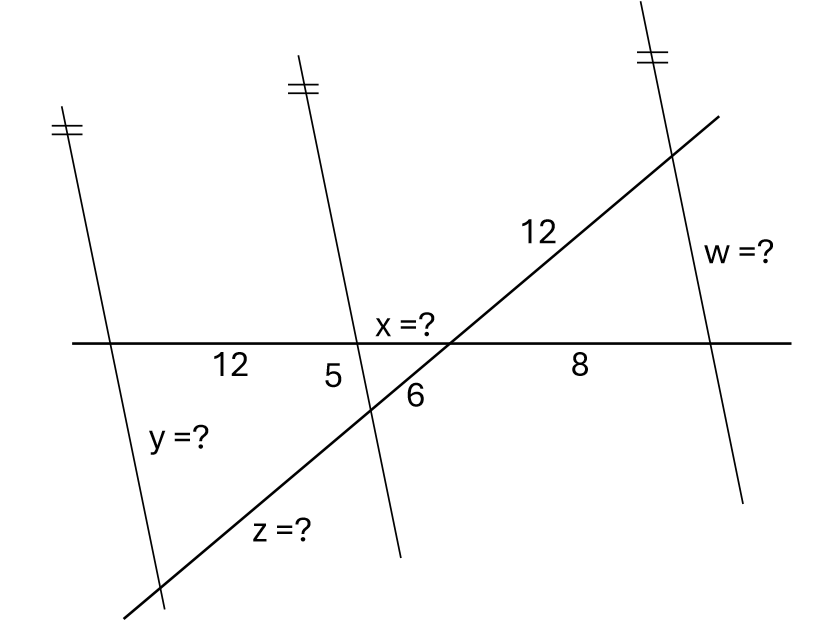
\includegraphics[scale=0.5]{Geometrie/data-geometrie/GZP25_Teil1Aufg4.png}
\end{figure}
\ifthenelse{\boolean{printanswers}}
{\begin{solution}
		tbd
\end{solution}}
{}

%------------------------------------------------
\newpage
\noaddpoints
\question[\totalpoints]
\addpoints
\begin{minipage}{0.4\linewidth}
	\begin{parts}
		\part[1] Bestimme $\displaystyle\frac{A_2}{A_1}$
		\part[1] Bestimme $\displaystyle\frac{A_3}{A_1}$
	\end{parts}
\end{minipage}
\hfill
\begin{minipage}{0.55\linewidth}
	\centering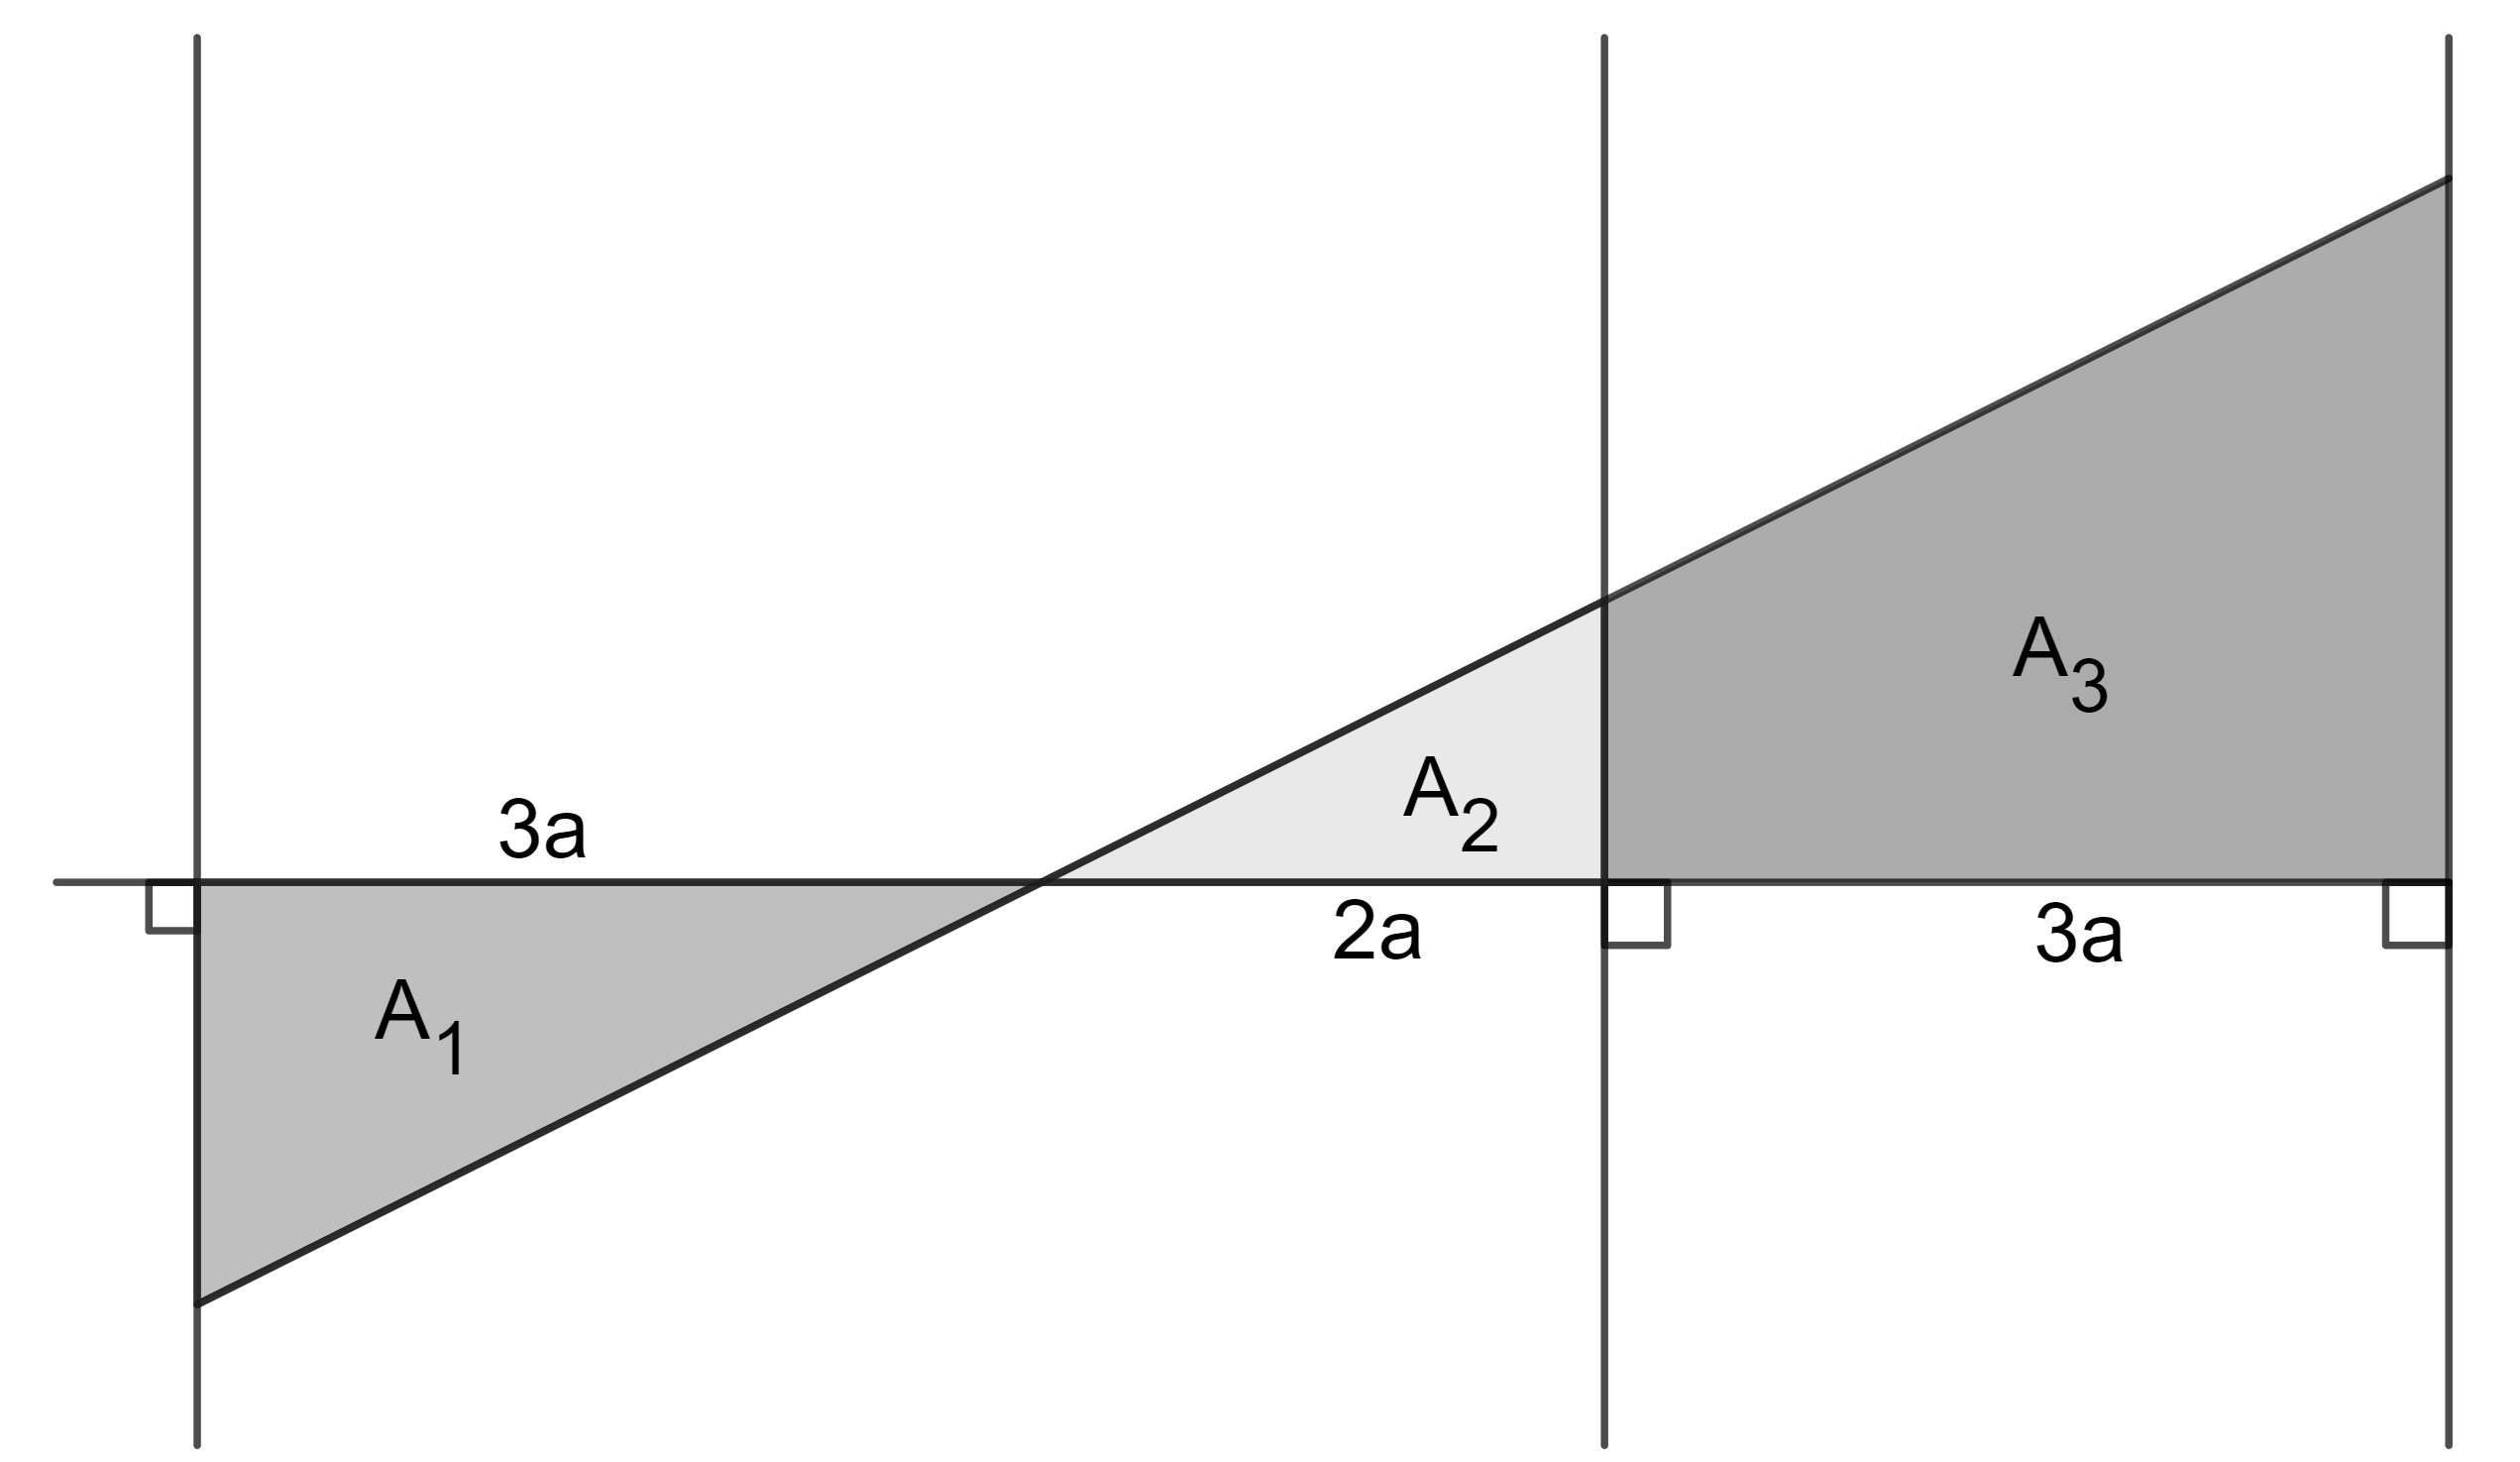
\includegraphics[scale=0.18]{Geometrie/data-geometrie/GZP25_Teil1Aufg5.png}
\end{minipage}
\ifthenelse{\boolean{printanswers}}
{\begin{solution}
		tbd
\end{solution}}
{\antwort{9}}


\question[3]
Entscheide in der Tabelle unten, ob die Gleichungen richtig oder falsch sind. Die Antworten müssen nicht begründet werden.\newline
\begin{small}
	Bewertung: Für $0-2$ korrekte Antworten gibt es keine Punkte; $3$ korrekte Antworten $1.5$ Punkt und falls alle Antworten korrekt sind, gibt es $3$ Punkte.\newline
\end{small}
\begin{minipage}{0.35\linewidth}
	\centering
	\begin{tikzpicture}[cross/.style={draw, cross out, minimum size=2*(#1-1pt), inner sep=0pt, outer sep=0pt}, x=10mm, y=10mm, 
		>=latex,   %Voreinstellung für Pfeilspitzen
		font= \footnotesize, scale=2.4]
		%Raster zeichnen
		% \draw [color=gray!50]  [step=5mm] (-1.1,-1.1) grid (1.1,1.1);
		% Achsen zeichnen
		\draw[->,thick] (-1.1,0) -- (1.2,0) node[right, below] {\normalsize $x$};
		\draw[->,thick] (0,-1.1) -- (0,1.2) node[above, left] {\normalsize $y$};
		% Achsen beschriften
		\foreach \x in {-1,1} \draw (\x,-.03) -- (\x,.03) node[below=4pt] {$\x$};
		\foreach \y in {-1,1} \draw (-.03,\y) -- (.03,\y) node[left=4pt] {$\y$};
		% Besserer Ursprung
		\draw[color=black] (0pt,-3pt) node[right] {$0$};
		%Funktionen zeichnen:
		\clip(-1.1,-1.1) rectangle (1.1,1.1); %Bildbereich
		\draw circle [radius=1];
	\end{tikzpicture}
\end{minipage}
\hfill
\begin{minipage}{0.6\linewidth}
	\begingroup
	\renewcommand{\arraystretch}{1.5}
	\begin{table}[H]
		\centering
		\begin{tabular}{|p{6cm}|c|c|}\hline
			& richtig & falsch \\\hline
			$\displaystyle\tan{125^\circ}<0$ & & \\\hline
			$\displaystyle\sin{\alpha}=\sin{180^\circ-\alpha}$ & & \\\hline
			$\displaystyle\cos{34'^\circ}=\cos{200^\circ}$ & & \\\hline
			$\displaystyle\cos{10^\circ}\*\tan{10^\circ}=\sin{10^\circ}$ & & \\\hline
		\end{tabular}
	\end{table}
	\endgroup
\end{minipage}


%------------------------------------------------
\newpage
\noaddpoints
\question[\totalpoints]
\addpoints
Berechne die Lösungsmenge der folgenden Gleichungen für $x$.
\begin{parts}
	\part[2] $11-6(x-14)=20-3(2x-25)$
\end{parts}
\ifthenelse{\boolean{printanswers}}
{\begin{solution}
		tbd
\end{solution}}
{\vspace{5pt}\antwort{4.5}}
\begin{parts}
	\setcounter{partno}{1}
	\part[2] $(x^2-7x+10)(7x-1)=0$
\end{parts}
\ifthenelse{\boolean{printanswers}}
{\begin{solution}
		tbd
\end{solution}}
{\vspace{5pt}\antwort{5}}
\begin{parts}
	\setcounter{partno}{2}
	\part[2] $2x^2+3=7x$
\end{parts}
\ifthenelse{\boolean{printanswers}}
{\begin{solution}
		tbd
\end{solution}}
{\vspace{5pt}\antwort{5}}
\begin{parts}
	\setcounter{partno}{3}
	\part[2] $\displaystyle\frac{x-1}{x+3}-\frac{x-4}{x+5}=\frac{7x+13}{x^2+8x+1}$
\end{parts}
\ifthenelse{\boolean{printanswers}}
{\begin{solution}
		tbd
\end{solution}}
{\vspace{5pt}\antwort{5}}


%------------------------------------------------
\newpage
\question[4]
Löse das Gleichungssystem ohne Diskussion der Sonderfälle.
\[\systeme{ax+2y=4,x+y=a}\]
\ifthenelse{\boolean{printanswers}}
{\begin{solution}
		tbd
\end{solution}}
{\antwort{20}}

%------------------------------------------------
\newpage
\noaddpoints
\question[\totalpoints]
\addpoints
\begin{minipage}{0.47\linewidth}
	\begin{parts}
		\part[2] Gib die Funktionsgleichung der dargestellten Gerade $a$ an.
		\part[1] Zeichne die Gerade $b:y=2x-1$ ins Koordinatensystem ein.
	\end{parts}
\end{minipage}
\hfill
\begin{minipage}{0.47\linewidth}
	\centering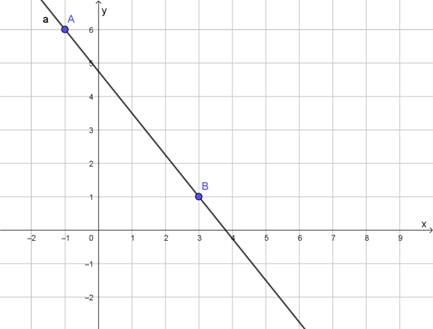
\includegraphics[scale=0.6]{Geometrie/data-geometrie/GZP25_Teil1Aufg9.png}
\end{minipage}
\begin{parts}
	\setcounter{partno}{2}
	\part[2] Bestimme die Gleichung der zu $b$ senkrechten Gerade $c$, die durch den Punkt $P(5,-7)$ geht.
	\part[2] Bestimme den Schnittpunkt der beiden Geraden $a$ und $b$.
\end{parts}
\ifthenelse{\boolean{printanswers}}
{\begin{solution}
		tbd
\end{solution}}
{\vspace{5pt}\antwort{17}}


\endgradingrange{ersterTeil} % beendet die Unterteilung der Notentabelle
\end{questions}



%=========================================================
%------------------- TEIL ZWEI
%=========================================================
\newpage
\thispagestyle{empty}
\noindent
\begin{tabular*}{\textwidth}{l @{\extracolsep{\fill}}l @{\extracolsep{7pt}}l}
     Kanton St. Gallen & & \multirow{4}{4em}{
\includegraphics[scale=0.2]{../Header/wappen_sg.png}}\\
     Bildungsdepartement & & \\
     & & \\
     \textbf{Kantonsschule Heerbrugg} & & \\
\end{tabular*}
\vspace{1cm}\newline
\begingroup
\renewcommand{\arraystretch}{1.5}
\begin{tabular*}{\textwidth}{l @{\extracolsep{\fill}}l @{\extracolsep{6pt}}l}\hline
    \textbf{\theme} & {\bf Lehrpersonen:} & Dc, Fh, Gt, Gu, Ss \\\hline
    \textbf{Mathematik, Teil 2 (mit TR)} & {\bf Dauer:} & {\bf 45 Minuten} \\\hline
    \textbf{Name:} & {\bf Klasse:} &  \\\hline
    \textbf{Vorname:} &  & \\\hline
\end{tabular*}
\endgroup

\begin{center}
    \textbf{Bewertungstabelle}\\
    {\small Wird von der Lehrperson ausgefüllt}\\
    \vspace{10pt}
    \addpoints
    \partialgradetable{zweiterTeil}[h][questions]\\[1cm]
    Der Rechenweg muss \textbf{vollständig und nachvollziehbar} sein. \\
    Unvollständige Lösungswege haben einen Punktabzug zur Folge.\\
    Als Hilfsmittel ist nur ein Taschenrechner (Ti-30X o.a.) erlaubt.\\
\end{center}

\noindent
\rule[1ex]{\textwidth}{1pt}

\vfill
\begin{center}
    %\Huge{Repetitionsprüfung}
\end{center}
%========================================================

\newpage
\begin{questions}
\setcounter{question}{9} % fixiert den counter für fortlaufende Nummerierung
\begingradingrange{zweiterTeil} % beginnt die Unterteilung der Notentabelle
%=========================================================
%-------------------TESTFRAGEN
%=========================================================
\question[3]
Berechne $x$ und $y$.
\begin{figure}[H]
	\centering\includegraphics[scale=0.8]{Geometrie/data-geometrie/GZP25_Teil2aufg1.png}
\end{figure}
\ifthenelse{\boolean{printanswers}}
{\begin{solution}
		tbd
\end{solution}}
{\vspace{5pt}\antwort{8}}
\vfill
\question[3]
\begin{minipage}{0.45\linewidth}
	In einem rechtwinkligen Dreieck mit der Hypothenuse $c=10$ cm unterscheiden sich die Kathetenquadrate um $20$ cm$^2$.\\ Berechne die Höhe $h_c$.
\end{minipage}
\hfill
\begin{minipage}{0.52\linewidth}
	\centering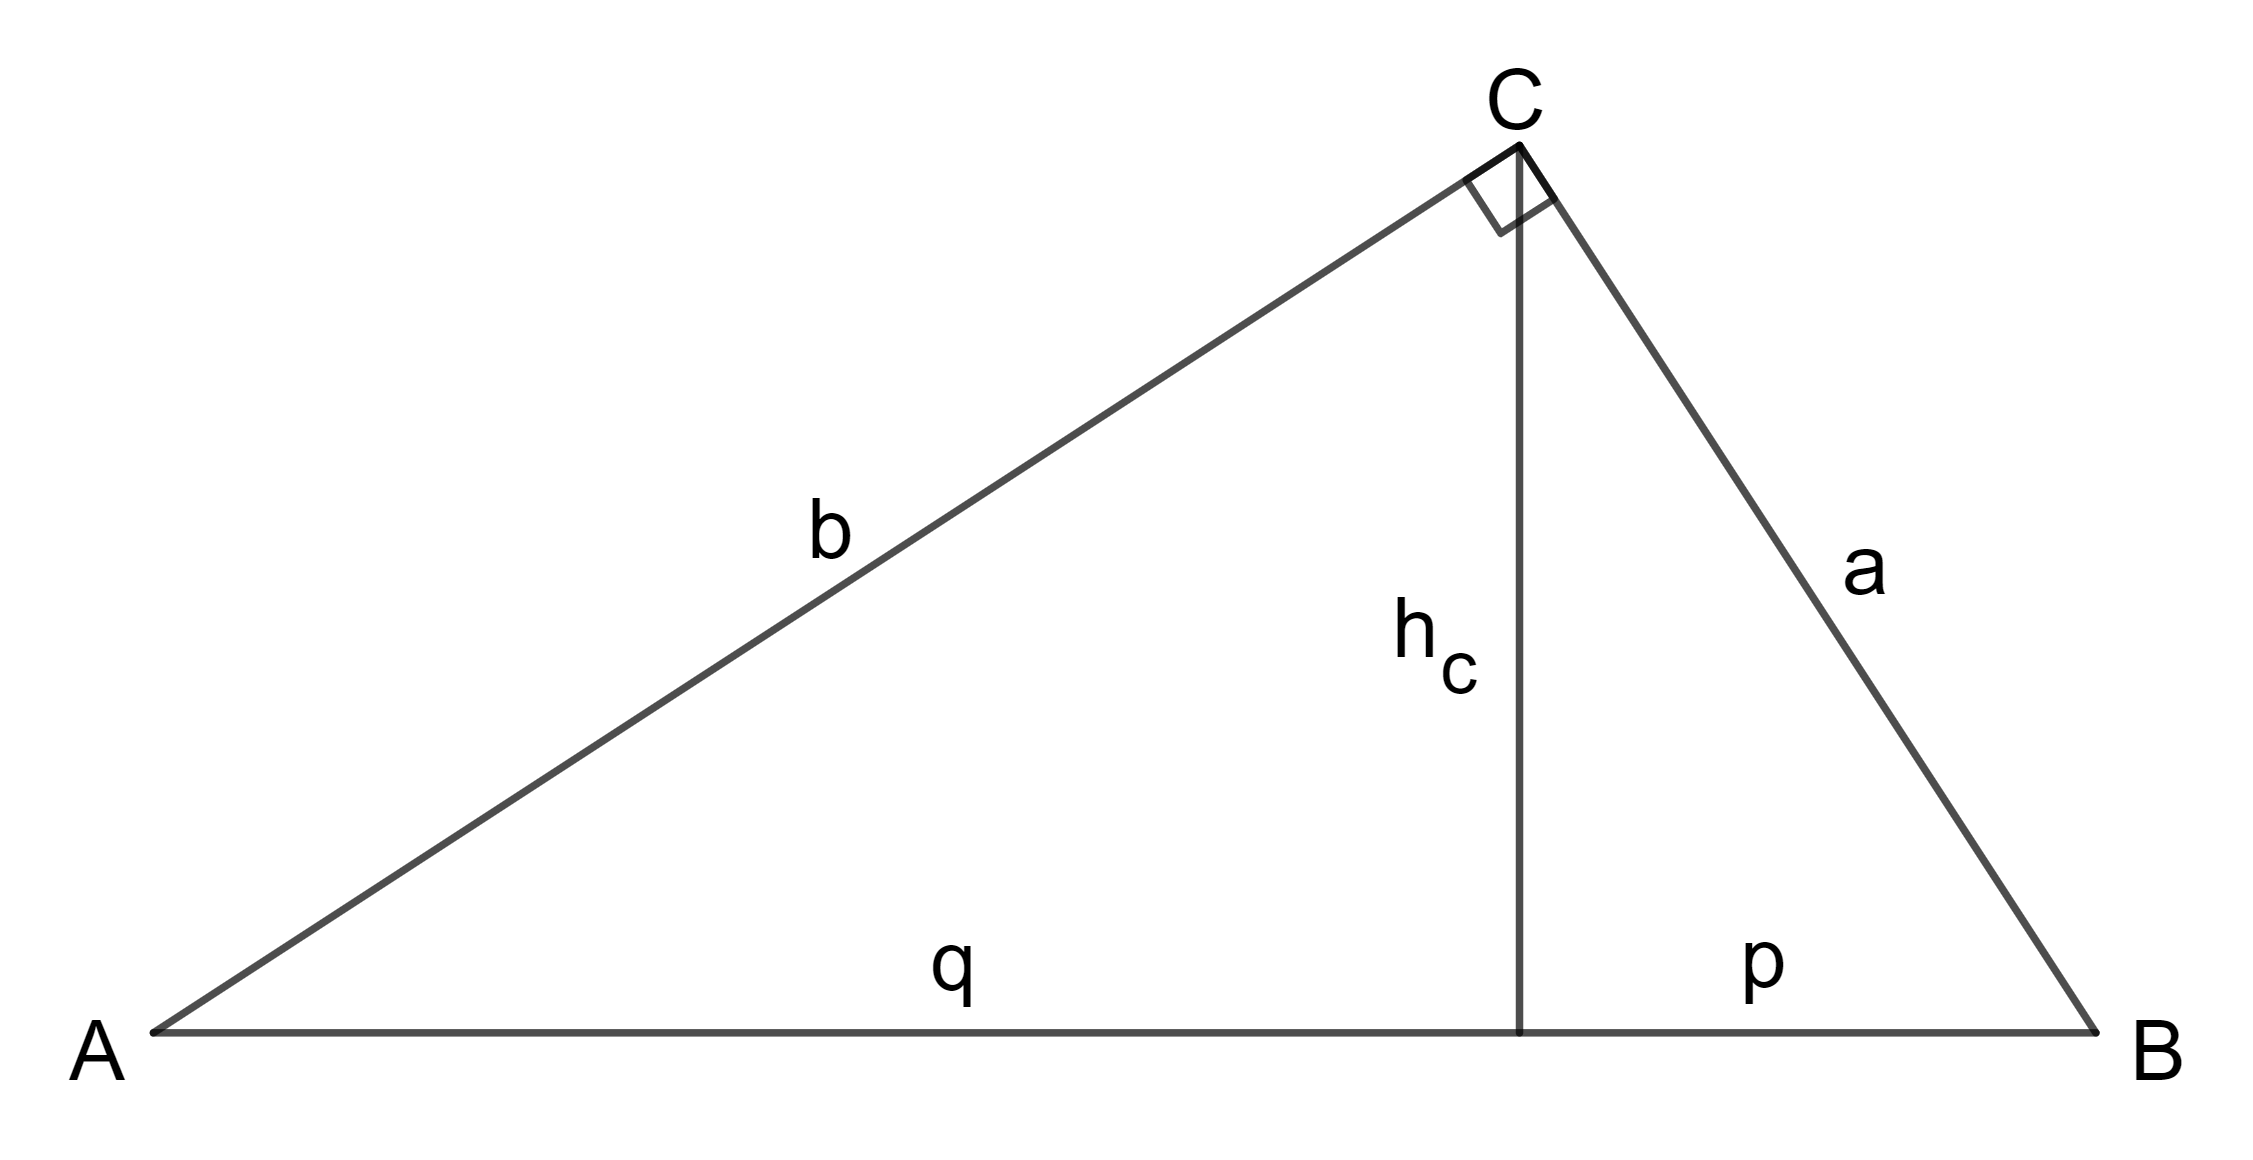
\includegraphics[scale=0.2]{Geometrie/data-geometrie/GZP25_Teil2Aufg2.png}
\end{minipage}
\ifthenelse{\boolean{printanswers}}
{\begin{solution}
		tbd
\end{solution}}
{\vspace{5pt}\antwort{8}}


%------------------------------------------------
\newpage
\question[4]
Die Katheten eines rechtwinkligen Dreiecks messen $a=3.7$ und $b=2.4$ Berechne die Länge der Winkelhalbierenden des Winkel $\alpha$.
\ifthenelse{\boolean{printanswers}}
{\begin{solution}
		tbd
\end{solution}}
{\vspace{5pt}\antwort{9}}
\vfill
\question[4]
\begin{minipage}{0.47\linewidth}
	Berechne die Berghöhe $h$ aus den Angaben $\alpha=42^\circ$ und $\beta=59^\circ$.
\end{minipage}
\hfill
\begin{minipage}{0.47\linewidth}
	\centering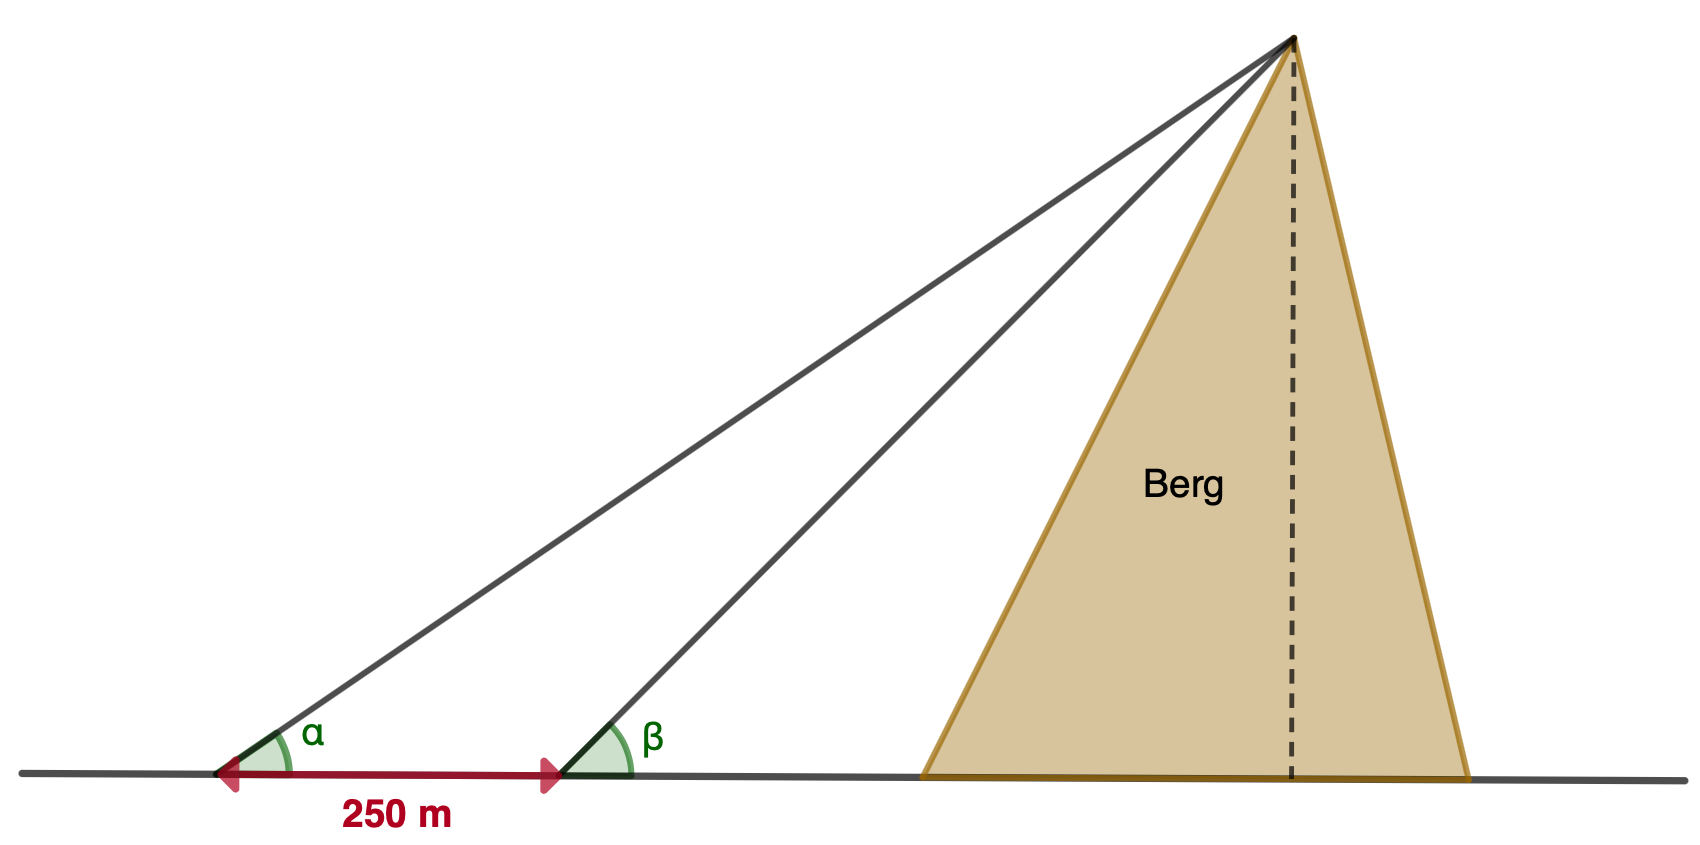
\includegraphics[scale=0.5]{Geometrie/data-geometrie/GZP25_Teil2Aufg4.png}
\end{minipage}
\ifthenelse{\boolean{printanswers}}
{\begin{solution}
		tbd
\end{solution}}
{\vspace{5pt}\antwort{9}}


%------------------------------------------------
\newpage
\noaddpoints
\question[\totalpoints]
\addpoints
\begin{parts}
	\part[3] Bestimme die Gleichung $y=ax^2+bx+c$ einer quadratischen Funktion mit den Nullstellen $x_1=2$ und $x_2=4$ so, dass die Parabel durch den Punkt $P(-1/30)$ geht.
	\part[1] Gib die Koordinaten des Scheitelpunktes an.
\end{parts}
\ifthenelse{\boolean{printanswers}}
{\begin{solution}
		tbd
\end{solution}}
{\vspace{5pt}\antwort{22}}


%------------------------------------------------
\newpage
\question[2]
\begin{minipage}{0.65\linewidth}
	In einer geraden, quadratischen Säule misst die Seite des Grundquadrates $1$ m. Die Körperdiagonale $d=\overline{AB}$ ist um $40\%$ kürzer als der kürzeste Weg $k$, auf dem man allein über die Kanten von $A$ nach $B$ gelangen kann.\\ Berechne die Höhe der Säule $h$.
\end{minipage}
\hfill
\begin{minipage}{0.3\linewidth}
	\centering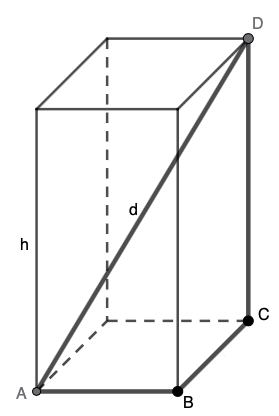
\includegraphics[scale=0.6]{Geometrie/data-geometrie/GZP25_Teil2Aufg6.png}
\end{minipage}
\ifthenelse{\boolean{printanswers}}
{\begin{solution}
		tbd
\end{solution}}
{\vspace{5pt}\antwort{21}}


%------------------------------------------------
\newpage
\question[6]
Die Parabel mit der Gleichung $y=ax^2+bx+c$ hat den Scheitelpunkt $S(-1/5)$ und schneidet die Gerade $g:y=5x-43$ bei $x=3$. Berechne den zweiten Schnittpunkt der Parabel mit der Geraden.
\ifthenelse{\boolean{printanswers}}
{\begin{solution}
		tbd
\end{solution}}
{\vspace{5pt}\antwort{23}}

%------------------------------------------------
\newpage
\noaddpoints
\question[\totalpoints]
\addpoints
Thomas steht gerne früh auf und fährt gerne Velo. Um $06:40$ Uhr startet er jeweils und fährt mit konstanter Geschwindigkeit an die Kanti. Er wohnt $7.5$ km von der Schule entfernt und kommt jeweils um $07:25$ Uhr an. Sein Kollege Franz, der weiter weg wohnt, fährt manchmal mit ihm, aber heute morgen hat er verschlafen. Franz nimmt deshalb das Töffli, mit dem er konstante $40$ km/h fahren kann, und rast um $07:10$ Uhr am Haus von Thomas vorbei.
\begin{parts}
	\part[2] Kann Franz Thomas noch einholen?
	\part[4] Wenn ja, um welche Uhrzeit holt er Thomas ein und wie viele Kilometer sind sie noch von der Schule entfernt?\newline\ \newline Wenn nein, kommt Franz noch rechtzeitig zum Unterricht zur Schule?
\end{parts}
\ifthenelse{\boolean{printanswers}}
{\begin{solution}
		tbd
\end{solution}}
{\vspace{5pt}\antwort{18}}

\endgradingrange{zweiterTeil} % beendet die Unterteilung der Notentabelle

\end{questions}
\end{document}